\phantomsection
\chapter{Face detection}

\noindent Face detection is the first step after image acquisition. It represents a requirement for a Facial Expression Recognition system. All the background is not taken into account. It allows to focus only on what is interesting in the input image: the face, which helps reducing the processing during the next step that is feature extraction.
\newline

\phantomsection
\section{Detection}

\vspace{\baselineskip}
\noindent Finding out if the input image or video sequence represents or contains a particular object is what is called Detection. Usually after the detection step comes the recognition step. For this system, the recognition step consists in facial expression recognition. But depending on the recognition, there can be another step that is the tracking step. Tracking consists in following a moving target on the images of a video sequence \cite{DIN08}.
\newline

\noindent To represent an object detector, the term "black box" can be used. The box gets an image as its input and at a high level the output can be considered as an image with annotations saying where the object of interest appears, if it appears \cite{DIN08}. For example, the output can look like in figure~\ref{output_example_face_detection} \cite{DIN08}.
\newline

\begin{figure}[!h]
\begin{center}
\noindent 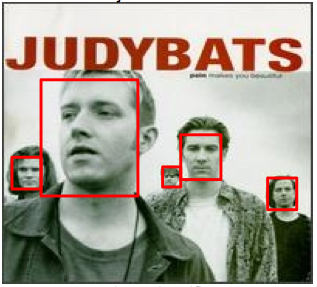
\includegraphics[scale=0.7]{figures/output_example_face_detection} 
\newline
\caption{Example of an output of face detection}
\label{output_example_face_detection}
\end{center} 
\end{figure}

\noindent But at a low level, the output is not anymore an annotated image. The object detector has a basic component that is something required to say if an instance of the object of interest is contained in a certain region or sub-region of the original image or not. This is what a binary classifier does \cite{DIN08}. For example, what a binary classifier does can look like in figure~\ref{output_example_face_detection_binary_classifier} \cite{DIN08}.
\newline

\begin{figure}[!h]
\begin{center}
\noindent 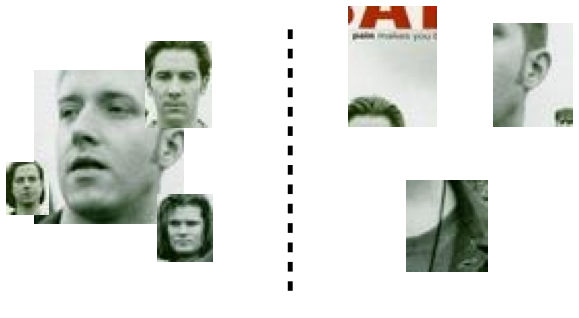
\includegraphics[scale=0.5]{figures/output_example_face_detection_binary_classifier} 
\newline
\caption{Example of what does a binary classifier for face detection}
\label{output_example_face_detection_binary_classifier}
\end{center} 
\end{figure}

\phantomsection
\section{Classifiers}

\vspace{\baselineskip}
\noindent Classification aim to solve the problem of identifying in a set of categories or sub-populations to which a new observation belongs. It is based on a training set of data that contains instances whose category affiliations are known. A classifier is an algorithm that implements classification. Classifiers groups data into categories. This can be done based on some measures of inherent similarity; for example, vectors represent the distance between instances, ad this in a multidimensional vector space \cite{CLASS}.
\newline









